\documentclass[conference]{IEEEtran}
\usepackage[T1]{fontenc}
\usepackage{amsmath,amssymb}
\usepackage{booktabs}
\usepackage{multirow}
\usepackage{graphicx}
\usepackage{xcolor}
\usepackage[hidelinks]{hyperref}


\begin{document}

\title{Do Spiking Networks Help Flow-Based Intrusion Detection? A Duplicate-Controlled Comparison on CSE-CIC-IDS2018}

\author{\IEEEauthorblockN{\"Ozg\"ur U\c{c}ar}
\IEEEauthorblockA{ucar45ozgur@gmail.com}}

\maketitle

\begin{abstract}
Spiking neural networks (SNNs) are proposed for network intrusion detection because neuromorphic hardware could run them at low power, but most reported results come from random row splits of duplicate-heavy benchmarks without tree baselines. We revisit the question on CSE-CIC-IDS2018 (16.2 million flows, 13 classes). Rows with identical feature vectors stay in one partition, fitting, calibration, threshold selection and testing use five disjoint partitions, and every model is judged at the same benign false-alarm rate (FAR). We compare a three-branch ensemble SNN with a parameter-matched multilayer perceptron (MLP), the same MLP on a spike-free piecewise-linear encoding, a spike-input control that feeds the SNN's encodings to a non-spiking network, and tree ensembles. Over five seeds at a 5\% FAR, the 4-step SNN reaches a macro-F1 of $0.766 \pm 0.011$, against $0.755$ for the MLP, $0.761$ for the piecewise-linear MLP, $0.779$ for the spike-input control and $0.808$ for XGBoost. Only the gap to XGBoost is significant. We find no evidence that spiking dynamics add accuracy: at the 5\% budget the SNN is equivalent to the piecewise-linear MLP within 2 points, and the non-spiking spike-input control has the highest neural mean. Four time steps match twelve at 2.9 times fewer synaptic events, yet on published Loihi costs it needs about 3\,$\mu$J per flow, 2.5 times the MLP's 1.24\,$\mu$J with SRAM weight reads. As reported for conventional detectors, frozen models transfer poorly to CIC-IDS2017, detecting 23\%--32\% of attack flows after threshold recalibration, and 13.5\%--34.4\% when retrained without the destination port. Code and records are released.
\end{abstract}

\begin{IEEEkeywords}
intrusion detection, spiking neural networks, CSE-CIC-IDS2018, data leakage, cross-dataset evaluation, neuromorphic computing
\end{IEEEkeywords}

\section{Introduction}

Network intrusion detection systems (NIDS) that classify flow records are attractive because flow export is cheap and already deployed in most networks. Learning-based detectors trained on public benchmarks such as CSE-CIC-IDS2018~\cite{sharafaldin2018} routinely report accuracies above 99\%. Spiking neural networks~\cite{maass1997} have joined this line of work, motivated by the low power that neuromorphic chips such as Loihi~\cite{davies2018,davies2021} promise for always-on monitoring.

Two problems make many of these numbers hard to interpret. The CIC datasets contain labelling and feature-extraction errors~\cite{engelen2021,liu2022,flood2024}, and a large share of their rows are exact duplicates. When a random row split puts copies of the same vector into both training and test sets, the test score partly measures memorisation~\cite{kaufman2012,arp2022}. SNN papers also tend to compare against convolutional or recurrent networks trained in a similar way, while gradient-boosted trees, which remain hard to beat on tabular data~\cite{grinsztajn2022,shwartzziv2022}, are left out. Reporting accuracy at the default argmax decision hides the operating point that matters to an analyst, namely how many attacks are caught at a fixed rate of false alarms~\cite{apruzzese2023sok}.

This paper asks a narrow question. If the evaluation keeps duplicate vectors out of the test set, calibrates every model the same way and fixes the false-alarm rate, does an ensemble SNN offer an accuracy or efficiency advantage on CSE-CIC-IDS2018? Our contributions are:

\begin{itemize}
\item A duplicate-controlled protocol for CSE-CIC-IDS2018, with separate partitions for model selection, probability calibration, alarm calibration and test, applied here to SNN-based detection.
\item A spike-input control that feeds the SNN's encodings to a non-spiking network. Together with a parameter-matched MLP and three tree ensembles, it separates the contribution of the encoding from that of the membrane dynamics. At five seeds we find no evidence that the dynamics add accuracy, and at the 5\% budget the SNN is equivalent within 2 points to an MLP on a spike-free piecewise-linear encoding.
\item An audit of duplicated feature vectors that quantifies how much of the remaining error comes from vectors carrying conflicting labels, extending earlier analyses of labelling errors in this dataset~\cite{liu2022}.
\item A time-window ablation ($T \in \{4,8,12\}$) with energy estimates under two cost models, which disagree on whether the SNN is cheaper than the MLP.
\item A transfer test of the frozen detectors on CIC-IDS2017 and a label-budget study of local adaptation, which confirm for SNNs the cross-dataset failure reported for other learners~\cite{dhooge2023sensors,cantone2024}.
\end{itemize}

Our results are mixed. The SNN is a competent detector and runs with a third of its time window at no measurable loss, but it does not reach the tree ensembles, and we cannot distinguish it from a non-spiking network fed the same encoded input.

\section{Related Work}

\textbf{Dataset quality and cross-dataset tests.} Engelen et al.~\cite{engelen2021} documented flow-construction and labelling errors in CIC-IDS2017, Lanvin et al.~\cite{lanvin2023} showed that such errors change detection results, and Liu et al.~\cite{liu2022} extended the analysis to CSE-CIC-IDS2018. Flood et al.~\cite{flood2024} catalogue structural design problems in benchmark NIDS datasets. Others list evaluation pitfalls~\cite{arp2022,sommer2010} and argue for deployment-oriented assessment~\cite{apruzzese2023sok}. Cross-dataset failure is well documented here. D'hooge et al. trained on CSE-CIC-IDS2018 and tested on CIC-IDS2017 and related sets~\cite{dhooge2023sensors}, and studied the reverse direction~\cite{dhooge2023jcp}; supervised models rarely learned a representation that carried over. Cantone et al.~\cite{cantone2024} ran a systematic cross-dataset study over CIC-IDS2017, CSE-CIC-IDS2018 and their corrected versions. Our transfer test repeats this kind of experiment for SNNs.

\textbf{Tabular baselines and numerical encodings.} Tree ensembles still match or beat deep networks on most tabular benchmarks~\cite{grinsztajn2022,shwartzziv2022}. Gorishniy et al.~\cite{gorishniy2022} showed that piecewise-linear and periodic embeddings of scalar features substantially improve plain MLPs. Deterministic spike codes of a scalar are, in effect, fixed binning or radial-basis encodings, so a gain from spike encoding may be an instance of this effect.

\textbf{Spiking networks and energy.} Surrogate-gradient training~\cite{neftci2019} made it practical to train SNNs with backpropagation through time, and snnTorch~\cite{eshraghian2023} brought this into standard tooling. Patel et al.~\cite{patel2026spiketiming} found that for intrusion detection the choice of spike code matters more than the neuron model. Energy claims for SNNs usually rest on an accumulate costing less than a multiply-accumulate~\cite{horowitz2014}. Dampfhoffer et al.~\cite{dampfhoffer2023} showed with a hardware-aware model that includes memory access that SNNs beat efficient ANN implementations only at high spike sparsity. Loihi figures are given in~\cite{davies2018,davies2021}.

\textbf{SNN-based intrusion detection.} Zhou and Li~\cite{zhou2021singlespike} compared single-spike temporal-coded networks with tree-ensemble figures taken from earlier work. Wang et al.~\cite{wang2024convsnn} reported 98.82\% accuracy for a convolutional SNN on a six-class subset of CSE-CIC-IDS2018 without a described split, against neural baselines only. Others use NSL-KDD, BoT-IoT or random splits~\cite{zivadinovic2024resource,fesu2025comparative,karthik2026hybrid}. Patel et al.~\cite{patel2026spiketiming} benchmarked 27 spiking configurations under capture-aware splits, without non-spiking baselines. Hardware evidence comes from a TrueNorth chip~\cite{alom2017truenorth} and an FPGA~\cite{mehrabi2024industrial}. Our contribution is to bring controls that the NIDS evaluation literature already recommends (duplicate-aware splits, tree baselines, fixed false-alarm operating points and cross-dataset tests) to SNN-based detection, and to add a spike-input control. Where Patel et al. ask which code works best, the control asks whether spiking adds anything beyond the code.

\textbf{Calibration and operating points.} We use class-prior correction~\cite{saerens2002} and temperature scaling~\cite{guo2017}, and set alarm thresholds in the Neyman--Pearson framing~\cite{tong2018}; unlike the umbrella algorithm of Tong et al., our empirical-quantile threshold has no finite-sample guarantee.

\section{Data and Protocol}

\begin{figure*}[t]
\centering
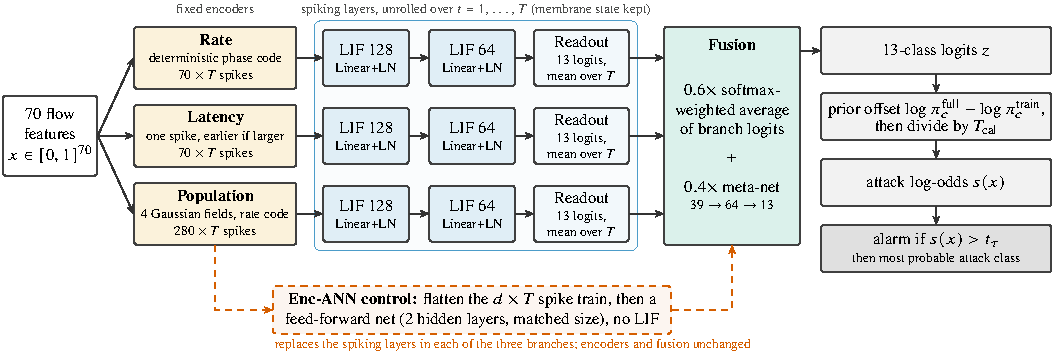
\includegraphics[width=\textwidth]{figures/fig_architecture}
\caption{Ensemble SNN. Three fixed encoders turn the 70 scaled flow features into spike trains over $T$ steps, each branch passes them through two LIF layers and a time-averaged readout, and the branch logits are fused before the prior offset, temperature $T_\mathrm{cal}$ and alarm threshold $t_\tau$ are applied. The time window $T$ and the temperature $T_\mathrm{cal}$ are unrelated. The dashed path is the spike-input control (Enc-ANN), which replaces the spiking layers with a feed-forward network on the flattened spike train.}
\label{fig:arch}
\end{figure*}

\subsection{Dataset and cleaning}

We use the ten daily CSV files of CSE-CIC-IDS2018 from Kaggle (\texttt{solarmainframe/} \texttt{ids-intrusion-csv}). After removing repeated header lines and rows with unparseable timestamps, 16{,}232{,}929 flows remain. Original labels are mapped to 13 classes; the three web-attack labels (brute force, XSS and SQL injection) are merged into one \emph{Web Attacks} class because together they have only 928 flows. Flow identifiers, IP addresses, source port and timestamp are dropped before learning. Non-finite values are set to zero.

\subsection{Feature-group split}

We compute a 128-bit fingerprint of each row's cleaned feature vector and treat all rows with the same fingerprint as one group. Groups, not rows, are assigned to training, tuning, calibration and test partitions in a 60/10/10/20 ratio (split seed 2026). This guarantees only that no test vector was seen verbatim in training, not that near-duplicates from one attack episode are separated, hence ``duplicate-controlled''. Classes with many duplicates shrink a great deal under this rule. DDoS-HOIC, for example, has 686{,}012 flows but only 198{,}861 distinct vectors. Table~\ref{tab:data} gives the resulting support.

The training partition is capped at 500{,}000 rows. Classes with at most 10{,}000 training rows are kept in full, and the remaining capacity is shared in proportion to class size. No synthetic oversampling is used. The calibration partition is split again by groups, half for fitting probability calibration and half for choosing alarm thresholds, which gives five disjoint partitions in total.

\begin{table}[t]
\centering
\caption{Support per class after the feature-group split. Per-class ratios deviate from 60/10/10/20 because whole duplicate groups go to one partition. Only training is capped.}
\label{tab:data}
\setlength{\tabcolsep}{3pt}
\begin{tabular}{lrrrr}
\toprule
Class & Train (capped) & Tune & Cal. & Test \\
\midrule
Benign & 335{,}515 & 1{,}362{,}310 & 1{,}330{,}511 & 2{,}699{,}900 \\
Bot & 16{,}651 & 22{,}981 & 33{,}237 & 54{,}821 \\
DDoS-HOIC & 26{,}260 & 68{,}256 & 69{,}218 & 134{,}836 \\
DDoS-LOIC-UDP & 1{,}066 & 159 & 181 & 324 \\
DDoS-LOIC-HTTP & 23{,}516 & 57{,}929 & 57{,}319 & 115{,}366 \\
DoS-GoldenEye & 10{,}601 & 4{,}135 & 4{,}078 & 8{,}362 \\
DoS-Hulk & 20{,}762 & 46{,}577 & 45{,}539 & 92{,}601 \\
DoS-SlowHTTPTest & 14{,}486 & 6{,}487 & 568 & 11{,}441 \\
DoS-Slowloris & 6{,}422 & 1{,}053 & 1{,}064 & 2{,}451 \\
FTP-BruteForce & 16{,}781 & 1{,}879 & 6{,}095 & 7{,}049 \\
Infiltration & 13{,}497 & 16{,}205 & 16{,}432 & 32{,}470 \\
SSH-BruteForce & 13{,}887 & 9{,}435 & 9{,}888 & 61{,}742 \\
Web Attacks & 556 & 87 & 106 & 179 \\
\bottomrule
\end{tabular}
\end{table}

\subsection{Preprocessing}

Every preprocessing step is fitted on the training partition only. Constant columns are removed, columns with absolute skew above 5 get a signed $\log(1+|x|)$ transform, and a quantile transformer maps each feature to $[0,1]$. Seventy features remain.

\subsection{Decision rule}

All models output 13 class scores $z$, which we treat as logits (tree ensembles use log-probabilities). Because training was class-capped, we add a prior offset~\cite{saerens2002}, $\tilde z_c = z_c + \log \pi_c^{\mathrm{full}} - \log \pi_c^{\mathrm{train}}$. A single temperature $T_\mathrm{cal}$ is then fitted by minimising negative log-likelihood on up to 100{,}000 rows of the probability-calibration half~\cite{guo2017}. The alarm score is the attack log-odds
\begin{equation}
s(x) = \log \sum_{c \neq \mathrm{B}} e^{\tilde z_c/T_\mathrm{cal}} - \tilde z_\mathrm{B}/T_\mathrm{cal},
\end{equation}
where B denotes the benign class. We call the share of benign flows that raise an alarm the false-alarm rate (FAR) and the share of attack flows that raise an alarm the detection rate (DR). For a FAR budget $\tau$, the threshold $t_\tau$ is the empirical $(1-\tau)$ quantile of $s$ over benign rows of the alarm-calibration half. A flow raises an alarm if $s(x) > t_\tau$ and is then assigned the class $\arg\max_{c \neq \mathrm{B}} \tilde z_c$. We use $\tau \in \{1\%, 5\%, 10\%\}$ and fixed $\tau = 5\%$ as the primary budget before testing. Test labels are never used to pick a threshold, a temperature or a checkpoint.

\section{Models}

\textbf{Input.} Every model receives one static vector of 70 flow statistics per flow, as exported by CICFlowMeter. Besides durations, packet and byte counts, inter-arrival statistics and flag counts, the inputs include the destination port and the protocol number as numeric features; only the source port is dropped. Destination port is a known shortcut in testbed captures, since several attacks target a single service. Retraining without it (three seeds, $T = 4$, same partitions, compared with the three-seed runs that include it) costs one to three points of macro-F1 at the 5\% budget: 13-class E-SNN $0.766 \to 0.754$, Enc-ANN $0.787 \to 0.776$, XGBoost $0.808 \to 0.799$; on the 11 identifiable classes 2.0, 2.9 and 1.2 points (XGBoost Holm $p = 0.002$). The consistent losses are on DoS-Slowloris, Web Attacks and Bot, while the two label-conflicted classes move erratically. DR stays within 0.1 points and the ranking is unchanged. We therefore keep it as an input; its role in transfer is examined in Section~\ref{sec:transfer}. No model sees packet sequences; the SNN's time steps only encode each static value as a short spike train.

\textbf{Ensemble SNN (E-SNN).} Three branches (Fig.~\ref{fig:arch}) share the same architecture and differ only in how the 70 features become spikes over $T = 12$ time steps. The \emph{rate} branch uses a deterministic phase-accumulator code: feature $x$ adds $x$ to a phase each step and spikes when the phase crosses an integer, with a fixed golden-ratio offset per feature. The \emph{latency} branch emits a single spike at step $\mathrm{round}((1-x)(T-1))$, so larger values spike earlier. The \emph{population} branch expands each feature into four Gaussian receptive fields with centres evenly spaced on $[0,1]$ and width $1/3$, and rate-codes their activations. Each branch has two hidden layers of 128 and 64 leaky integrate-and-fire neurons (decay initialised at 0.9 and learned), layer normalisation before each spiking layer and dropout of 0.2, followed by a linear readout averaged over time. The branch outputs are combined as $0.6$ times a softmax-weighted average plus $0.4$ times a meta-network ($39 \to 64 \to 13$). This mixture was fixed in an earlier version of the study and not tuned here. The model has 86{,}013 parameters and is trained with surrogate gradients (fast sigmoid, slope 25) in snnTorch~\cite{eshraghian2023}.

\textbf{Matched MLP.} A perceptron with two hidden layers of 252 units (layer normalisation, GELU, dropout 0.2), a width chosen by parameter count alone to match the E-SNN (85{,}945 parameters). It sees the quantile-scaled features directly.

\textbf{Spike-input control (Enc-ANN).} The same three fixed encoders and fusion head as the E-SNN, but each branch flattens the whole spike train and passes it through a two-hidden-layer feed-forward network whose width matches the parameter count of the corresponding SNN branch (84{,}503 parameters at $T = 12$). Because the flattened input grows with $T$, the hidden width shrinks (21, 21 and 13 units for the rate, latency and population branches at $T = 12$; 53, 53 and 39 at $T = 4$). Comparing E-SNN with Enc-ANN separates the effect of the encoding from the effect of membrane dynamics.

\textbf{Spike-free encoding control (PLE-MLP).} A two-hidden-layer MLP on a 16-bin piecewise-linear encoding of each feature~\cite{gorishniy2022}. The bins are uniform on the quantile-scaled input, so they are training-set quantile bins. Matching the parameter count (85{,}923) on the 1{,}120-dimensional input leaves 71 hidden units, against 252 for the matched MLP, so capacity and encoding are not fully separated. It is a single network without the three-branch fusion of the E-SNN and Enc-ANN.

\textbf{Tree ensembles.} Random forest~\cite{breiman2001} (200 trees, depth 25), XGBoost~\cite{chen2016} (400 trees, depth 8, learning rate 0.1, row and column subsampling 0.8, histogram method) and CatBoost~\cite{prokhorenkova2018} (600 iterations, depth 8, learning rate 0.05). These are common defaults and were not tuned. The neural models, in contrast, were early-stopped on tuning data and the E-SNN went through a five-variant screen, so the neural side received more tuning effort.

\textbf{Training details.} All neural models use AdamW with learning rate $4\times10^{-4}$, weight decay $10^{-3}$, batch size 1{,}024, gradient-norm clipping at 1.0 and plain cross-entropy, for at most 35 epochs. We keep the checkpoint with the best prior-corrected macro-F1 on the tuning partition and stop after 10 epochs without improvement. The main run trains every model for three seeds (42, 43, 44) at $T = 12$. A second run on the same partitions trains the E-SNN, Enc-ANN, matched MLP, PLE-MLP and XGBoost at $T = 4$ with five seeds (42--46) and is our primary evidence for model comparisons; its seeds 42--44 reproduce the earlier runs exactly (MLP and XGBoost at $T = 12$, E-SNN and Enc-ANN at $T = 4$), so only seeds 45 and 46 are new. We moved the primary comparison to $T = 4$ and added the PLE-MLP to the declared comparisons after the second review round, when $T = 4$ and $T = 12$ were already known to perform alike on test. Seeds change initialisation and batch order, not the split. As a further check, the E-SNN and matched MLP were also trained with class-weighted cross-entropy. The full configuration is in \texttt{configs/group\_ce.json}.

Follow-up experiments reuse the partitions, preprocessor and decision rule byte for byte; the code refuses to run if data hashes or package versions differ. They retrain the E-SNN and Enc-ANN at $T = 4$ and 8 (three seeds) and screen five E-SNN variants.

\section{Results}
\label{sec:results}

\subsection{Detection at a fixed FAR budget}

\begin{table}[t]
\centering
\caption{Test results at a 5\% FAR budget (mean $\pm$ s.d.). Top: $T = 4$, five seeds (primary). Bottom: $T = 12$, three seeds. Trees do not depend on $T$; the top XGBoost row adds seeds 45--46. MF1-11 excludes FTP-BruteForce and DoS-SlowHTTPTest (Section~\ref{sec:errors}). DR and FAR are seed means.}
\label{tab:main}
\setlength{\tabcolsep}{2.5pt}
\begin{tabular}{lcccc}
\toprule
Model & Macro-F1 & MF1-11 & DR & FAR \\
\midrule
\multicolumn{5}{l}{\emph{$T = 4$, five seeds}} \\
E-SNN & $0.766 \pm 0.011$ & $0.828 \pm 0.014$ & $0.959$ & $0.049$ \\
Matched MLP & $0.755 \pm 0.004$ & $0.820 \pm 0.004$ & $0.958$ & $0.050$ \\
PLE-MLP & $0.761 \pm 0.005$ & $0.824 \pm 0.003$ & $0.959$ & $0.049$ \\
Enc-ANN & $0.779 \pm 0.020$ & $0.842 \pm 0.013$ & $0.961$ & $0.049$ \\
XGBoost & $0.808 \pm 0.004$ & $0.858 \pm 0.001$ & $0.967$ & $0.049$ \\
\midrule
\multicolumn{5}{l}{\emph{$T = 12$, three seeds}} \\
E-SNN & $0.769 \pm 0.022$ & $0.837 \pm 0.019$ & $0.959$ & $0.049$ \\
Matched MLP & $0.756 \pm 0.004$ & $0.821 \pm 0.005$ & $0.958$ & $0.050$ \\
Enc-ANN & $0.787 \pm 0.017$ & $0.848 \pm 0.017$ & $0.963$ & $0.049$ \\
Random forest & $0.788 \pm 0.001$ & $0.842 \pm 0.001$ & $0.965$ & $0.050$ \\
CatBoost & $0.791 \pm 0.005$ & $0.843 \pm 0.004$ & $0.965$ & $0.049$ \\
XGBoost & $0.808 \pm 0.005$ & $0.858 \pm 0.001$ & $0.967$ & $0.049$ \\
\bottomrule
\end{tabular}
\end{table}

The achieved test FAR is 4.9\% to 5.0\% for every model (Table~\ref{tab:main}), and the KS distance between benign calibration and test scores is 0.005 to 0.014.

All models catch about 96\% of attack flows, and DR spans only 0.9 points. More than 99\% of the missed attack flows are Infiltration, so DR says little about the models. The separation shows up in macro-F1, which weights rare and difficult classes equally. We test four declared comparisons for the E-SNN on the five-seed $T = 4$ run (Welch, Holm within each metric and budget; the XGBoost gap at 5\% also survives Holm over all 16 tests). At the 5\% budget the E-SNN differs from the matched MLP by $+1.1$ points (95\% CI $[-0.3, 2.5]$, Holm $p = 0.32$), from the PLE-MLP by $+0.5$ ($[-0.9, 1.9]$, $p = 0.51$), from Enc-ANN by $-1.3$ ($[-3.8, 1.2]$, $p = 0.51$) and from XGBoost by $-4.2$ ($[-5.6, -2.8]$, $p = 0.002$). At 1\% only the XGBoost gap is significant ($-5.2$, $[-7.3, -3.1]$, $p = 0.007$), as on the 11 identifiable classes ($-3.0$ at 5\%, $p = 0.031$; $-4.2$ at 1\%, $p = 0.041$). With five seeds a Welch test has 80\% power for gaps of about 2 points against the MLP and PLE-MLP and 3.4 points against Enc-ANN. The three-seed $T = 12$ run gives the same picture (Holm $p \geq 0.25$ at 5\%). These intervals cover seed variance; the split seed is fixed.

For equivalence we use a 2-point margin, the five-seed MDE80, chosen in the third review round after the data were seen. TOST shows the E-SNN equivalent to the PLE-MLP at the 5\% budget ($p = 0.020$; 11 classes $p = 0.031$), but not at 1\% ($p = 0.087$) and not to the MLP ($p = 0.074$); the PLE-MLP is itself equivalent to the MLP at 5\% ($p = 0.001$), in line with its 71-unit capacity limit. In exploratory comparisons Enc-ANN is 2.4 and 3.7 points above the MLP at 5\% and 1\% (90\% CIs exclude zero) and 1.8 to 2.2 above the PLE-MLP. We thus find no evidence that spiking dynamics add accuracy; whether the Enc-ANN's edge comes from the spike codes or its three-branch fusion is not resolved. An approximate bootstrap over the 2.29 million test fingerprint groups (200 replicates) holds models and thresholds fixed, so it excludes threshold-refit variance. Its intervals are narrow (E-SNN DR 95.89\% [95.47, 96.46], FAR 4.91\% [4.84, 4.98] at 5\%), and every paired DR and AUC difference keeps its sign (E-SNN minus XGBoost: $-0.84$ DR points, $[-0.93, -0.72]$). These binary gaps stay below one point while the macro-F1 gaps to XGBoost and Enc-ANN are several points, so those models differ mainly in which attack class they assign, not in whether they alarm. Macro-F1 is not bootstrapped because per-row class predictions were not saved.

In the three-seed run the order at 1\% matches 5\%; at 10\% Enc-ANN (0.767) passes random forest (0.763). The prior-corrected argmax decision runs at a FAR of 0.02\% to 0.14\% with higher macro-F1 than the 5\% budget for every model except random forest. The prior offset carries the whole calibration effect; fitted temperatures lie between 0.96 and 1.01. Class-weighted training did not help (E-SNN 0.753, MLP 0.747).

Per capture day the FAR ranges from 0.1\% to 24.1\% for the E-SNN and up to 32.3\% for XGBoost, exceeding 15\% for every model on the two Infiltration days, plausibly because of unlabelled malicious traffic~\cite{liu2022}.

\subsection{Where the errors are}
\label{sec:errors}

Table~\ref{tab:perclass} lists per-class F1. Eight of the thirteen classes are detected almost perfectly (F1 $\geq 0.96$) by every model. The differences between models come from the other five: DDoS-LOIC-UDP, DoS-SlowHTTPTest, FTP-BruteForce, Infiltration and Web Attacks.

\begin{table}[t]
\centering
\caption{Per-class test F1 at a 5\% FAR budget, $T = 12$, mean of three seeds. The eight classes with F1 $\geq 0.96$ for every model are omitted (DoS-Slowloris, for example, ranges from 0.964 for the E-SNN to 0.998 for XGBoost).}
\label{tab:perclass}
\setlength{\tabcolsep}{2.2pt}
\begin{tabular}{lcccccc}
\toprule
Class & E-SNN & MLP & Enc-ANN & RF & CatB. & XGB \\
\midrule
DDoS-LOIC-UDP & 0.821 & 0.816 & 0.821 & 0.869 & 0.850 & 0.837 \\
DoS-SlowHTTPTest & 0.552 & 0.519 & 0.625 & 0.747 & 0.757 & 0.734 \\
FTP-BruteForce & 0.243 & 0.271 & 0.274 & 0.234 & 0.255 & 0.337 \\
Infiltration & 0.127 & 0.124 & 0.152 & 0.169 & 0.166 & 0.171 \\
Web Attacks & 0.360 & 0.171 & 0.393 & 0.319 & 0.345 & 0.464 \\
\bottomrule
\end{tabular}
\end{table}

The feature-group audit explains part of this. All 193{,}360 FTP-BruteForce flows fall into just 54 distinct vectors, and 193{,}353 of them lie in groups that also carry another label. For DoS-SlowHTTPTest, 139{,}884 of 139{,}890 flows share vectors with other classes, and the three largest groups in the dataset mix these two classes. Both attacks leave short, nearly empty TCP connections that the flow extractor summarises identically, consistent with the labelling problems Liu et al. report~\cite{liu2022}. No classifier can separate such flows, and since whole groups go to one partition, the test F1 of these two classes mostly reflects how a few large groups fell in the split. Removing the two classes (MF1-11 in Table~\ref{tab:main}) narrows the gap between the E-SNN and random forest from 1.9 to 0.5 points and, at $T = 12$, puts Enc-ANN above random forest and CatBoost (at $T = 4$ it ties random forest at 0.842), so much of the 13-class ranking rests on these two classes. Infiltration is spread over 140{,}610 groups, and 88{,}810 of its rows lie in groups that also carry another label.

Across the whole dataset, 68{,}467 groups carry conflicting labels, and a classifier that predicts the majority label of each group would still be wrong on 1.10\% of rows. Since identical inputs cannot be separated even by memorisation, a lower error on these features implies a different label set or preprocessing, not leakage, and is not comparable with ours.

Web Attacks has high ROC AUC (0.994 for the seed-42 E-SNN, 1.000 for XGBoost) but low F1, because its 179 test flows face 2.7 million benign ones: the E-SNN finds 98 of them with 661 false assignments, XGBoost 160 with 342. Average precision (0.49 and 0.85) reflects this better than AUC.

\subsection{Operation counts and energy}

We counted operations with forward hooks on flows from four capture days and weighted the per-class counts by test-partition support. The eight classes measured cover 92\% of test rows. A linear layer with binary input costs one accumulate (AC) per nonzero input and output neuron; other layers cost multiply-accumulates (MACs).


At $T = 12$ the E-SNN's hidden neurons are silent 72\% of the time, yet with 12 steps and three branches it still performs four times as many synaptic events as the MLP performs MACs. With 45\,nm costs (0.9\,pJ per AC, 4.6\,pJ per MAC) the E-SNN's linear layers alone cost 0.33\,$\mu$J at $T = 12$, below the MLP's linear layers (0.39\,$\mu$J). Its layer normalisation and membrane updates run at every time step, though, and with them the E-SNN costs 0.49\,$\mu$J, about 23\% above the MLP's 0.40\,$\mu$J; at $T = 4$ it stays 55\% below. With SRAM weight reads the E-SNN costs more than the MLP at every $T$ (1.41 against 1.24\,$\mu$J at $T = 4$). Enc-ANN is far cheaper than both because it processes each binary input once instead of propagating it through membrane state. On one CPU thread the E-SNN is 40 to 50 times slower than the MLP (57 against 1.4\,$\mu$s per flow, and 105 against 2.1 in a repeat).

\begin{table}[t]
\centering
\caption{Operations and estimated energy per flow ($\mu$J), seed 42, test class mix. 45\,nm includes layer normalisation and membrane updates~\cite{horowitz2014}; +SRAM adds one SRAM read per weight use; INT8 ignores the wider membrane accumulator; Loihi uses published costs~\cite{davies2018}.}
\label{tab:loihi}
\small
\setlength{\tabcolsep}{2pt}
\begin{tabular}{lcrrrrrr}
\toprule
Model & $T$ & ACs & MACs & 45\,nm & +SRAM & INT8 & Loihi \\
\midrule
E-SNN & 4 & 120{,}028 & 3{,}367 & 0.18 & 1.41 & 0.007 & 3.1 \\
E-SNN & 8 & 233{,}577 & 3{,}367 & 0.33 & 2.70 & 0.013 & 6.0 \\
E-SNN & 12 & 347{,}762 & 3{,}367 & 0.49 & 4.00 & 0.019 & 9.0 \\
Enc-ANN & 4 & 31{,}349 & 12{,}352 & 0.09 & 0.53 & 0.004 & -- \\
Enc-ANN & 8 & 31{,}034 & 6{,}568 & 0.06 & 0.44 & 0.003 & -- \\
Enc-ANN & 12 & 30{,}153 & 5{,}094 & 0.05 & 0.41 & 0.002 & -- \\
MLP & -- & 0 & 84{,}420 & 0.40 & 1.24 & 0.020 & -- \\
\bottomrule
\end{tabular}
\end{table}

On Loihi each synaptic event (a spike times its fan-out) costs 23.6\,pJ and each neuron update 81\,pJ~\cite{davies2018}. The E-SNN then needs 3.1 to 9.0\,$\mu$J per flow, 2.5 to 7.2 times the like-for-like MLP cost with SRAM weight reads, which Loihi's per-event figure also includes (7.8 to 22.5 times the arithmetic-only 45\,nm cost). Under INT8 arithmetic the E-SNN is cheaper than the MLP at $T = 4$ and 8 and at parity at $T = 12$ (0.019 against 0.020\,$\mu$J). Over 90\% of the E-SNN total is synaptic events, three quarters of them from the input encoding; input injection, static power and routing are not costed.

\subsection{Shorter time windows}

Fig.~\ref{fig:steps} repeats the neural comparison with 4 and 8 time steps on the same partitions. For the E-SNN, three-seed macro-F1 at the 5\% budget is $0.766$, $0.766$ and $0.769$ at $T = 4$, 8 and 12 ($0.791$, $0.800$, $0.789$ at 1\%), with no detectable difference; Enc-ANN reaches $0.787$, $0.800$ and $0.787$. With hidden sparsity of 72\% to 74\%, synaptic events fall 2.9-fold from $T = 12$ to 4. The 90\% CI of the $T = 4$ minus $T = 12$ difference at 5\% is $[-3.7, 3.1]$ points, so a 2-point effect is not excluded. Enc-ANN has the highest neural mean at every window, with seed ranges that overlap the E-SNN's.

\begin{figure}[t]
\centering
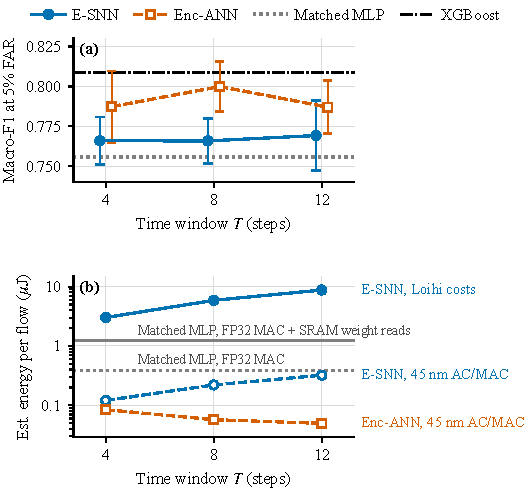
\includegraphics[width=\columnwidth]{figures/fig_steps}
\caption{Effect of the time window $T$. (a) Test macro-F1 at a 5\% FAR budget (mean and s.d.; diamonds: five seeds at $T = 4$, unconnected to the three-seed points at $T = 8$ and 12), with the five-seed MLP, PLE-MLP and XGBoost as references. (b) Estimated energy per flow on a log scale, as in Table~\ref{tab:loihi}: complete 45\,nm model, with SRAM reads, and Loihi costs for the E-SNN.}
\label{fig:steps}
\end{figure}

\subsection{Architecture screen}

Five E-SNN variants ($T = 8$, seed 42; wider layers, weighted-average fusion only, higher learning rate, eight receptive fields, population branch only) were ranked on tuning macro-F1 (0.775--0.833). On test they reached 0.753--0.768 against 0.756 for the original, all within its seed spread. The top-ranked wide variant, retrained with three seeds, reaches $0.770 \pm 0.014$ against $0.766 \pm 0.014$ for the original, with 2.5 times as many parameters. Per-variant results are in the records.

\subsection{Transfer to CIC-IDS2017}
\label{sec:transfer}

We ran the frozen seed-42 models, unchanged, on the CIC-IDS2017 MachineLearningCVE files from the Kaggle dataset \texttt{sweety18/cicids2017-full-dataset} (2{,}214{,}468 labelled flows). It was recorded a year earlier on another testbed with an older flow extractor. Our copy lacks the Tuesday and Thursday-morning files, so brute-force and web attacks are absent; the corrected releases~\cite{engelen2021,lanvin2023} would allow a fuller test. Columns are mapped by name (the map is released with the records); the protocol field is missing and is imputed from the destination port. Attack labels are mapped to the 2018 families; PortScan and Heartbleed have no 2018 counterpart. Against benign flows from four 2018 days, the median KS distance over the 70 inputs is 0.245. The largest shifts point to the extractor version: Fwd Seg Size Min (0.485), RST and ECE flags that are zero in 99.97\% of 2017 but 68\% of 2018 benign flows, and an initial backward window with median $-1$ against 149. Only 7 of the 70 inputs shift more across the datasets than between the two most different 2018 days, so network and extractor effects are mixed in the failure below.

\begin{table}[t]
\centering
\caption{Frozen 2018 models on CIC-IDS2017. ``Recal.'': threshold refitted on half of the 2017 benign flows (5\% budget), attack labels unused.}
\label{tab:transfer}
\setlength{\tabcolsep}{3.5pt}
\begin{tabular}{lcccc}
\toprule
& \multicolumn{2}{c}{2018 threshold} & \multicolumn{2}{c}{Recal.} \\
Model & FAR & DR & FAR & DR \\
\midrule
E-SNN ($T = 12$) & 0.262 & 0.630 & 0.050 & 0.230 \\
E-SNN ($T = 4$) & 0.228 & 0.420 & 0.050 & 0.239 \\
XGBoost & 0.252 & 0.494 & 0.050 & 0.317 \\
\bottomrule
\end{tabular}
\end{table}

Table~\ref{tab:transfer} confirms for SNNs the transfer failure reported for conventional learners on this dataset pair~\cite{dhooge2023sensors,dhooge2023jcp,cantone2024}. With the 2018 threshold the FAR rises from 5\% to 23\%--26\%. We then refitted each alarm threshold on half of the 2017 benign flows, the one adjustment possible without attack labels, and evaluated on the other half and on all attacks. DR then falls to 23\%--32\%. For the SNNs only the slow application-layer DoS attacks appear to transfer: the 12-step E-SNN still flags 86\% of GoldenEye and 87\% of Slowloris flows, and the 4-step E-SNN 99.8\% and 99.6\%, while XGBoost flags only 28.8\% of GoldenEye. This depends on the destination port. Retrained without it, the 4-step E-SNN flags 32.5\% of GoldenEye and 68.8\% of Slowloris flows. Removing the port does not repair transfer either: at the 2018 threshold the FAR is still 18\% (E-SNN) and 22\% (XGBoost), and after recalibration DR is 13.5\% and 31.0\%, against 23.9\% and 31.7\% with the port. The port-free Enc-ANN transfers best of all models tested (FAR 12.7\% at the 2018 threshold, recalibrated DR 34.4\%, ROC AUC 0.686), but this is still poor; its with-port counterpart was not calibrated locally. Fig.~\ref{fig:transfer} gives the recalibrated DR by attack type; no model detects Infiltration or Heartbleed.

\begin{figure}[t]
\centering
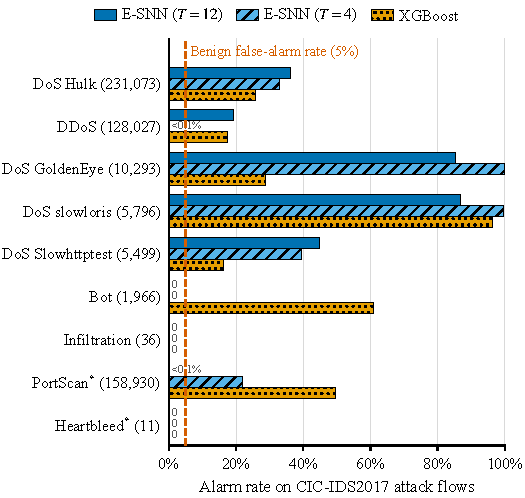
\includegraphics[width=0.8\columnwidth]{figures/fig_transfer}
\caption{Share of CIC-IDS2017 attack flows that raise an alarm after the threshold of each frozen 2018 model is refitted to a 5\% benign FAR (dashed line). Flow counts are in parentheses; an asterisk marks attack types with no CSE-CIC-IDS2018 counterpart.}
\label{fig:transfer}
\end{figure}

To estimate the local labels an operator would need, we split the CIC-IDS2017 flows by feature-vector fingerprint into an adaptation pool, a calibration partition and a test partition (50/10/40) and drew class-stratified labelled samples of 0.1\%, 1\% and 5\% of the pool (1{,}101, 11{,}026 and 55{,}153 flows). We call this the label budget, to distinguish it from the FAR budget. PortScan was added as a new class. The 5\% alarm threshold was refitted on about 83{,}000 known-benign flows of the 2017 calibration partition. Table~\ref{tab:adapt} fits the temperature on up to 100{,}000 labelled calibration flows; fitting it on the label budget alone, or dropping it, changes DR and FAR by at most 0.001, so the label count is the budget itself. Its frozen E-SNN runs at a 6.2\% FAR; at an exact 5\% test FAR it detects 24.8\%, close to the 23.9\% of Table~\ref{tab:transfer}.

\begin{table}[t]
\centering
\caption{Local adaptation on CIC-IDS2017 (test partition, mean over three seeds) by label budget, the labelled share of the adaptation pool. Budget 0 is the frozen 2018 model. All rows use a 5\% FAR threshold refitted on 2017 calibration data.}
\label{tab:adapt}
\setlength{\tabcolsep}{3pt}
\begin{tabular}{llcccc}
\toprule
Method & & 0 & 0.1\% & 1\% & 5\% \\
\midrule
\multirow{3}{*}{E-SNN $T{=}4$, fine-tuned} & FAR & 0.062 & 0.052 & 0.059 & 0.053 \\
 & DR & 0.268 & 0.985 & 0.994 & 0.996 \\
 & MF1 & 0.188 & 0.564 & 0.592 & 0.707 \\
\midrule
\multirow{3}{*}{XGBoost, from scratch} & FAR & 0.050 & 0.050 & 0.050 & 0.051 \\
 & DR & 0.314 & 0.996 & 1.000 & 1.000 \\
 & MF1 & 0.291 & 0.526 & 0.665 & 0.686 \\
\midrule
\multirow{3}{*}{XGBoost, continued} & FAR & -- & 0.051 & 0.050 & 0.057 \\
 & DR & -- & 0.723 & 0.724 & 0.749 \\
 & MF1 & -- & 0.510 & 0.494 & 0.483 \\
\bottomrule
\end{tabular}
\end{table}

With 1{,}101 labelled flows, fine-tuning the 4-step E-SNN from its 2018 checkpoint raises DR to 98.5\% at a 5.2\% FAR, and XGBoost trained from scratch on the same flows reaches 99.6\% at 5.0\% without any pre-training. At an equal test FAR of 1\% the gap widens to 95.9\% against 99.0\%. The fine-tuned E-SNN matches XGBoost on DoS, DDoS and PortScan traffic but not on Bot flows, which it misses with 0.1\% and 1\% of the pool and detects at 32\% with 5\%; XGBoost detects 97\% to 99.5\% of Bot flows with 1\% or more. Continuing the 2018 XGBoost model cannot learn PortScan and stays at 72\% to 75\% DR. Macro-F1 stays between 0.48 and 0.71 because a 5\% FAR on 671{,}643 benign test flows produces about 33{,}000 false alarms, which swamp the precision of the small classes. Pool and test share capture days and attack episodes, so this same-capture re-split is an optimistic bound; it shows that the data become easy once in-domain labels exist, not an SNN-specific effect.

\section{Discussion and Limitations}

\textbf{What the spikes buy.} Within this protocol we find no evidence that membrane dynamics add accuracy. Over five seeds the E-SNN is not separable from the matched MLP or from Enc-ANN, and at the 5\% budget it is equivalent within 2 points to an MLP on a spike-free piecewise-linear encoding~\cite{gorishniy2022}. Enc-ANN has the highest neural mean, though its difference from the E-SNN is not significant (Holm $p = 0.51$); it which feeds the same spike codes to a dense network and is cheaper under every cost model in Table~\ref{tab:loihi} that applies to it. Its edge over the MLP is exploratory, and we cannot tell whether it comes from the codes or from the three-branch fusion, since no fusion-matched PLE ensemble was trained. It does not rule out SNN advantages with on-chip encoding or on per-packet sequences, where time steps would be real time; that is the natural next experiment. SNN papers on flow features should include a spike-input control before crediting membrane dynamics.

\textbf{Energy needs a hardware model.} A 45\,nm adder cost favours the SNN at short windows when memory traffic is ignored; with SRAM reads, or with the published Loihi cost of a synaptic event, the MLP is cheaper at every $T$ (the E-SNN on Loihi costs 2.5 to 7.2 times the MLP with SRAM reads), mainly because the input encoding fans out to 128 neurons. This is an intrusion-detection instance of the sparsity threshold reported by Dampfhoffer et al.~\cite{dampfhoffer2023}. Energy claims should state their cost model.

\textbf{Trees remain strong.} Untuned XGBoost had the highest mean at every budget, in line with evidence on tabular data~\cite{grinsztajn2022,shwartzziv2022}, and a neuromorphic detector should be judged against it.

\textbf{Limitations.} The protocol was designed after test results of an earlier row-split version were seen, and later experiments followed the main test results. These are development results on one reused test partition, so we report every configuration we ran; a fresh held-out dataset is still needed. Feature groups prevent verbatim duplication but not near-duplicates or episode-level leakage within an attack run, and the dataset's timestamps are unverified, so we did not attempt a time-blocked split. Destination port is an input and acts as a shortcut worth one to three macro-F1 points. The five-seed run reuses the test partition, its primary role and the PLE-MLP comparison were fixed after review, and only two of its seeds are new. We used three or five seeds but a single split seed, so no interval covers a redrawn split; the group bootstrap covers test sampling for DR, FAR and AUC only. Tree hyperparameters were fixed, and we screened only five SNN variants. The CIC-IDS2017 copy is incomplete and was produced by an older extractor. All energy numbers are estimates from operation counts; we made no hardware measurements.

\section{Conclusion}

On CSE-CIC-IDS2018 under a duplicate-controlled protocol with matched false-alarm rates, an ensemble SNN detects 96\% of attack flows at a 5\% FAR. With five seeds we find no evidence that spiking dynamics add accuracy: at the 5\% budget it is equivalent within 2 points to a spike-free piecewise-linear MLP, it is not separable from the matched MLP, and a non-spiking network fed the same spike codes has the highest neural mean. XGBoost is about 4 points ahead (Holm $p = 0.002$). The SNN keeps its accuracy with 4 time steps instead of 12, which cuts its synaptic events by a factor of 2.9, but with published Loihi figures it still costs more energy per flow than the MLP. Much of the remaining error comes from identical vectors under different labels, and, as reported for other learners, no model carries its accuracy to CIC-IDS2017 without local labels, with or without the destination port.

\section*{Reproducibility}

Code, configuration, per-run records and the seed-42 checkpoints of the E-SNN ($T{=}4$ and 12), Enc-ANN ($T{=}12$), matched MLP and XGBoost are available at \url{https://github.com/ozgurucar/ids2018-ensemble-snn} (tag \texttt{paper-v1}). The remaining Kaggle outputs (other seeds, PLE-MLP and no-port checkpoints, per-row test scores) are available from the author on request and will be released with the camera-ready version. Training ran on a single Kaggle GPU; exact package versions are in \texttt{results/v3/requirements-run.lock.txt}. A Docker-packaged service serves the frozen checkpoints; all further results are in the per-run records.

\bibliographystyle{IEEEtran}
\bibliography{references}

\end{document}
